\documentclass[12pt]{report}
\usepackage[utf8]{inputenc}
\usepackage[russian]{babel}
%\usepackage[14pt]{extsizes}
\usepackage{listings}
\usepackage{graphicx}
\usepackage{amsmath,amsfonts,amssymb,amsthm,mathtools} 
\usepackage{pgfplots}
\usepackage{filecontents}
\usepackage{float}
\usepackage{indentfirst}
\usepackage{eucal}
\usepackage{enumitem}
%s\documentclass[openany]{book}
\frenchspacing

\usepackage{indentfirst} % Красная строка

\usetikzlibrary{datavisualization}
\usetikzlibrary{datavisualization.formats.functions}

\usepackage{amsmath}


% Для листинга кода:
\lstset{ %
	language=c,                 % выбор языка для подсветки (здесь это С)
	basicstyle=\small\sffamily, % размер и начертание шрифта для подсветки кода
	numbers=left,               % где поставить нумерацию строк (слева\справа)
	numberstyle=\tiny,           % размер шрифта для номеров строк
	stepnumber=1,                   % размер шага между двумя номерами строк
	numbersep=5pt,                % как далеко отстоят номера строк от подсвечиваемого кода
	showspaces=false,            % показывать или нет пробелы специальными отступами
	showstringspaces=false,      % показывать или нет пробелы в строках
	showtabs=false,             % показывать или нет табуляцию в строках
	frame=single,              % рисовать рамку вокруг кода
	tabsize=2,                 % размер табуляции по умолчанию равен 2 пробелам
	captionpos=t,              % позиция заголовка вверху [t] или внизу [b] 
	breaklines=true,           % автоматически переносить строки (да\нет)
	breakatwhitespace=false, % переносить строки только если есть пробел
	escapeinside={\#*}{*)}   % если нужно добавить комментарии в коде
}


\usepackage[left=2cm,right=2cm, top=2cm,bottom=2cm,bindingoffset=0cm]{geometry}
% Для измененных титулов глав:
\usepackage{titlesec, blindtext, color} % подключаем нужные пакеты
\definecolor{gray75}{gray}{0.25} % определяем цвет
\newcommand{\hsp}{\hspace{20pt}} % длина линии в 20pt
% titleformat определяет стиль
\titleformat{\chapter}[hang]{\Huge\bfseries}{\thechapter\hsp\textcolor{gray75}{|}\hsp}{0pt}{\Huge\bfseries}


% plot
\usepackage{pgfplots}
\usepackage{filecontents}
\usetikzlibrary{datavisualization}
\usetikzlibrary{datavisualization.formats.functions}

\begin{document}

	\begin{titlepage}
	\newgeometry{pdftex, left=2cm, right=2cm, top=2.5cm, bottom=2.5cm}
	\fontsize{12pt}{12pt}\selectfont
	\noindent \begin{minipage}{0.15\textwidth}
		
\includegraphics[width=\linewidth]{pictures/b_logo.jpg}
	\end{minipage}
	\noindent\begin{minipage}{0.9\textwidth}\centering
		\textbf{Министерство науки и высшего образования Российской Федерации}\\
		\textbf{Федеральное государственное бюджетное образовательное учреждение высшего образования}\\
		\textbf{«Московский государственный технический университет имени Н.Э.~Баумана}\\
		\textbf{(национальный исследовательский университет)»}\\
		\textbf{(МГТУ им. Н.Э.~Баумана)}
	\end{minipage}
	
	\noindent\rule{18cm}{3pt}
	\newline\newline
	\noindent ФАКУЛЬТЕТ $\underline{\text{«Информатика и системы управления»}}$ \newline\newline
	\noindent КАФЕДРА $\underline{\text{«Программное обеспечение ЭВМ и информационные технологии»}}$\newline\newline\newline\newline\newline\newline\newline
	
	
	\begin{center}
		\Large\textbf{Отчет по лабораторной работе №4}\newline
	\end{center}
	
	\noindent\textbf{Название} $\underline{\text{~Моделирование системы массового обслуживания~~~~~~~~~}}$\newline\newline\newline
	\noindent\textbf{Дисциплина} $\underline{\text{~Моделирование~~~~~~~~}}$\newline\newline
	\noindent\textbf{Студент} $\underline{\text{Золотухин А. В.~~~~~~~~~~~~~~~~~~~~~~~~~~~~~~~~~~~~~~~~~}}$\newline\newline
	\noindent\textbf{Группа} $\underline{\text{ИУ7-74Б~~~~~~~~~~~~~~~~~~~~~~~~~~~~~~~~~~~~~~~~~~~~}}$\newline\newline
	\noindent\textbf{Оценка (баллы)} $\underline{\text{~~~~~~~~~~~~~~~~~~~~~~~~~~~~~~~~~~~~~~~~~~~~~~~~~}}$\newline\newline
	\noindent\textbf{Преподаватель}$\underline{\text{~Рудаков И. В.~~~~~~~~~~}}$\newline
	
	\begin{center}
		\vfill
		Москва~---~\the\year
		~г.
	\end{center}
 \restoregeometry
\end{titlepage}


	\chapter{Задание}

	\section{Цель работы}

	\textbf{Цель работы:} построение гистограммы и эмпирической функции распределения.

	\section{Содержание работы}

	\begin{enumerate}
		\item Для выборки объёма $n$ из генеральной совокупности $X$ реализовать в виде программы на ЭВМ
			\begin{enumerate}
				\item вычисление максимального значения $M_{\max}$ и минимального значения $M_{\min}$;
				\item размаха $R$ выборки;
				\item вычисление оценок $\hat\mu$ и $S^2$ математического ожидания $MX$ и дисперсии $DX$;
				\item группировку значений выборки в $m = [\log_2 n] + 2$ интервала;
				\item построение на одной координатной плоскости гистограммы и графика функции плотности распределения вероятностей нормальной случайной величины с математическим ожиданием $\hat{\mu}$ и дисперсией $S^2$;
				\item построение на другой координатной плоскости графика эмпирической функции распределения и функции распределения нормальной случайной величины с математическим ожиданием $\hat{\mu}$ и дисперсией $S^2$.
			\end{enumerate}
		\item Провести вычисления и построить графики для выборки из индивидуального варианта.
	\end{enumerate}

\chapter{Теоретическая часть}

Пусть $\vec x$ -- выборка из генеральной совокупности $X$. 

\section{Формулы для вычисления величин}

\subsection{Минимальное и максимальное значения выборки}
\begin{equation}
    \begin{aligned}
        M_{\max} = x_{(n)}\\
        M_{\min} = x_{(1)}
    \end{aligned}\text{,}
\end{equation}
где $ x_{(n)}$ --- последнее значение вариационного ряда,

$x_{(1)}$ --- первое значение вариационного ряда.

\subsection{Размах выборки}
\begin{equation}
    R = M_{\max} - M_{\min}.
\end{equation}

\subsection{Оценки математического ожидания и дисперсии}
\begin{equation}
    \begin{aligned}
    \hat\mu(\vec X_n) &= \overline X_n = \frac 1n \sum_{i=1}^n X_i\\
    S^2(\vec X_n) & \frac 1{n-1} \sum_{i=1}^n (X_i-\overline X_n)^2
    \end{aligned}\text{,}
\end{equation}
где $\overline X_n$ --- выборочное среднее.
\section{Эмпирическая плотность и гистограмма}

При большом объеме $n$ этой выборки  значения $x_i$ группируют в интервальный статистический ряд. 

Отрезок $J = [x_{(1)}, x_{(n)}]$ делят на $m$ равновеликих частей.
\begin{equation}
	m=[\log_2n]+2\text{,}
\end{equation}
 где $n$ -- размер выборки.
\begin{equation}
    J_i = [x_{(1)} + (i - 1) \cdot \Delta, x_{(1)} + i \cdot \Delta), i = \overline{1; m - 1}
\end{equation}

\begin{equation}
    J_{m} = [x_{(1)} + (m - 1) \cdot \Delta, x_{(n)}]
\end{equation}

\begin{equation}
    \Delta = \frac{|J|}{m} = \frac{x_{(n)} - x_{(1)}}{m}
\end{equation}

\textbf{Интервальным статистическим рядом называют таблицу:}

\begin{table}[htb]
    \centering
    \begin{tabular}{|c|c|c|c|c|}
        \hline
        $J_1$ & ... & $J_i$ & ... & $J_m$ \\
        \hline
        $n_1$ & ... & $n_i$ & ... & $n_m$ \\
        \hline
    \end{tabular}
\end{table}

где $n_i$ -- количество элементов выборки $\vec x$, которые $\in J_i$.

\textbf{Эмпирической плотностью}, отвечающей выборке $\vec x$, называют функцию:
\begin{equation}
    \hat f(x) =
    \begin{cases}
        \frac{n_i}{n \Delta}, x \in J_i, i = \overline{1; m} \\
        0, \text{иначе} \\
    \end{cases}
\end{equation}

\textbf{Гистограмма} -- это график эмпирической плотности.

\section{Эмпирическаяя функция распределения}

Oбозначим $n(x, \vec x)$ -- число элементов выборки $\vec x$, которые имеют значения меньше $x$.

\textbf{Эмпирической функцией распределения} называют функцию $F_n: \mathbb{R} \to \mathbb{R}$, определенную как: 

\begin{equation}
    F_n(x) = \frac{n(x, \vec x)}{n}
\end{equation}

\chapter{Практическая часть}

\begin{lstlisting}[language=Matlab]
n = length(X);

M_max = max(X);
M_min = min(X);
fprintf("max = %f\n", X_max)
fprintf("min = %f\n", X_min)

R = M_max - M_min;
fprintf("R = %f\n", R)

MX = mean(X);
DX = var(X);
fprintf("MX = %f   DX = %f\n", MX, DX)

m = floor(log2(n)) + 2;
delta = R / m;
fprintf('m = %i  delta = %f\n', m, delta);

h = histogram(X, m);

sigma = sqrt(DX);
x = (M_min - 1):(sigma / 100):(M_max + 1);
f = normpdf(x, MX, sigma);

figure;
delta = h.BinWidth;
heights = h.Values / (n * delta);
centers = [];
for i = 1:m
centers = [centers, (h.BinEdges(i + 1) + h.BinEdges(i)) / 2];
end
hold on;
bar(centers, heights, 1); 
plot(x, f, 'LineWidth', 2);


F = normcdf(x, MX, sigma);
figure;
hold on;
[yy, xx] = ecdf(X);
xx = [xx; x_max + 1];
yy = [yy; 1];
plot(x, F, 'r');
\end{lstlisting}

\chapter{Экспериментальная часть}

\section{Результаты расчетов}

Выборка: X=[3.89,2.60,2.56,2.33,4.35,3.97,4.16,4.10,4.82,3.17,4.15,4.05,4.45,3.76,4.83,4.27,2.03,3.13,\\3.69,5.44,2.61,5.20,4.03,5.26,4.42,3.67,4.68,5.22,4.11,3.35,3.83,5.34,4.69,5.12,4.33,4.41,4.82,4.65,3.12,4.71,\\2.36,3.10,3.52,1.74,3.46,2.89,5.42,4.12,5.36,4.26,3.49,5.85,5.24,4.23,4.57,3.54,4.38,4.31,2.28,4.17,3.66,5.25,\\3.11,4.48,3.80,4.05,3.48,1.12,2.16,4.68,4.21,3.22,4.29,4.70,4.37,4.60,4.15,4.06,3.81,3.58,4.34,3.87,4.53,6.02,\\3.34,3.34,2.87,4.64,3.03,3.08,3.46,4.04,4.77,3.59,3.49,6.53,4.16,2.95,4.85,5.53,3.59,4.24,4.45,4.42,4.10,3.77,\\4.56,3.89,4.13,4.00,3.95,2.73,4.76,3.19,3.66,4.87,4.18,5.30,4.97,4.56];


Результаты работы программы для выборки (Вариант 4) представлены на рисунках.

\begin{figure}[ht!]	
	\centering{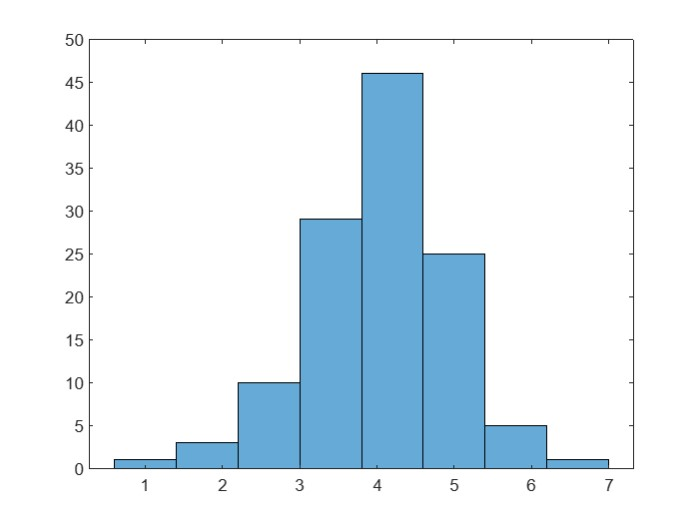
\includegraphics[width=0.7\textwidth]{res1.jpg}}
\end{figure}

\begin{figure}[ht!]	
	\centering{
		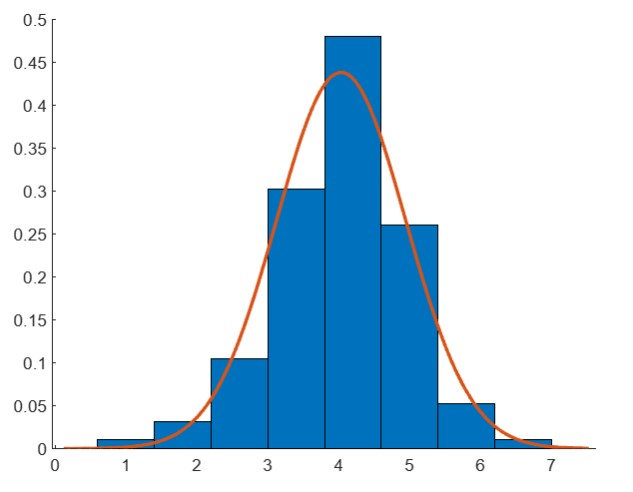
\includegraphics[width=0.6\textwidth]{res2.jpg}
		\caption{Гистограмма и график функции плотности распределения вероятностей нормальной случайной величины с выборочными мат. ожиданием и дисперсией}}
\end{figure}

\begin{figure}[ht!]	
	\centering{
		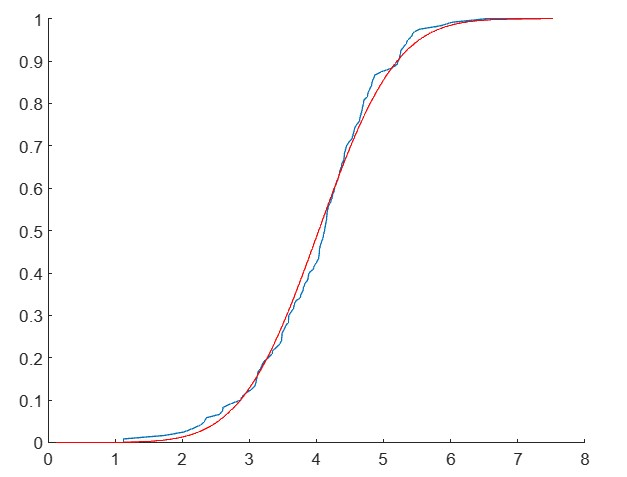
\includegraphics[width=0.6\textwidth]{res3.jpg}
		\caption{График эмперической функции распределения и функции распределения нормальной случайной величины с выборочными мат. ожиданием и дисперсией}}
\end{figure}

\end{document}
